%% Copyright 1998 Pepe Kubon
%%
%% `two.tex' --- 2nd chapter for thes-full.tex, thes-short-tex from
%%               the `csthesis' bundle
%%
%% You are allowed to distribute this file together with all files
%% mentioned in READ.ME.
%%
%% You are not allowed to modify its contents.
%%

%%%%%%%%%%%%%%%%%%%%%%%%%%%%%%%%%%%%%%%%%%%%%%%%%
%
%     Chapter 6  
%
%%%%%%%%%%%%%%%%%%%%%%%%%%%%%%%%%%%%%%%%%%%%%%%%

\chapter{Experiments}
\label{ch:exp}

In this chapter, we will evaluate our approach by reporting the experimental results with respect to the running time on computing the subspace skyline on both real data sets and synthetic data sets. We compare the running time of algorithm with and without using pruning method. Both of algorithms compute the subspace skyline using \emph{dominating candidate sets} enumerating framework. The only difference between the two program we compare is whether the pruning method has been applied to the algorithm.
We implement our algorithms using C++. We use Microsoft Visual Studio 2010 to compile our C++ programs. Experiments were conducted on a PC with an Intel Core(TM) i7-3779 3.40GHz CPU, 16GB main memory and a 900G hard disk, running the Microsoft Windows 7 Enterprise Edition operating system.

\section{Experiments of Skyline Subspace Query on Graph}

Using the model of Kronecker graph provided by~\cite{leskovec2005realistic}, we generated different sizes of graph.
According to~\cite{leskovec2005realistic}, Kronecker graph has the following real world network properties:
heavy tails for the in-degree and out-degree distribution;
heavy tails for the eigenvalues and eigenvectors;
small diameters; and the ``Densification Power Law" (DPL).
We use the MATLAB code from graph500 (\url{http://www.graph500.org/specifications#sec-3_3}) to generate the graph with scale from $15$ to $20$ which corresponds to the number of vertices from $2^{15}$ to $2^{20}$. All the graphs with different sizes are generated from the initial matrix:
\begin{equation}
\begin{bmatrix}
0.3 & 0.24\\ 
0.24 & 0.22
\end{bmatrix}
\end{equation}
with edge factor $2$ which is the expected average degree of the vertices. The label is generated in Pareto distribution which is a Power Law Distribution. We use the Pareto function from a python package numpy to generate the label information of the vertices. Figure~\ref{fig:exp:kronecker} shows running comparison between the algorithms with and without pruning.

\begin{figure}[h]
    \centering
      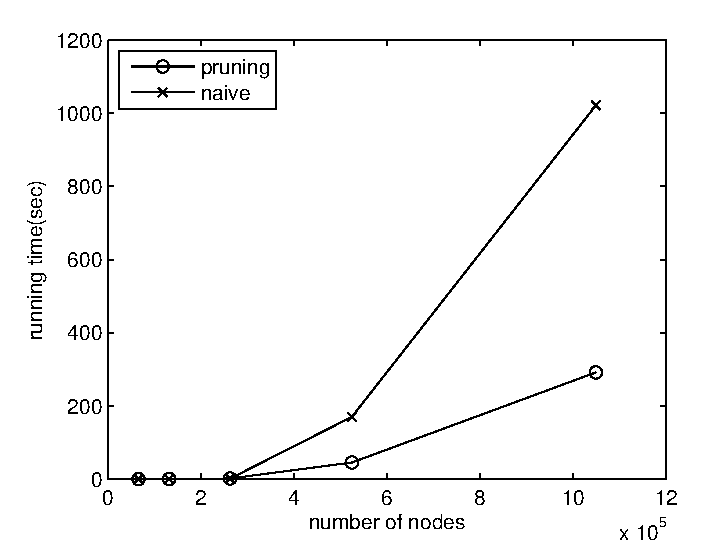
\includegraphics[width=0.7\textwidth]{figs/kronecker}
    \caption{\label{fig:exp:kronecker}Blue: Running time with pruning, Green: Running time without pruning}
\end{figure}



\begin{figure}[h]
    \centering
      \includegraphics[width=0.7\textwidth]{figs/FB}
    \caption{o: Running time with pruning, x: Running time without pruning}
\end{figure}

Facebook data set:\\
Graph: 4039 Nodes, 88234 Edges.\\
Label: 20 Labels in total.\\
    
\begin{figure}[h]
    \centering
      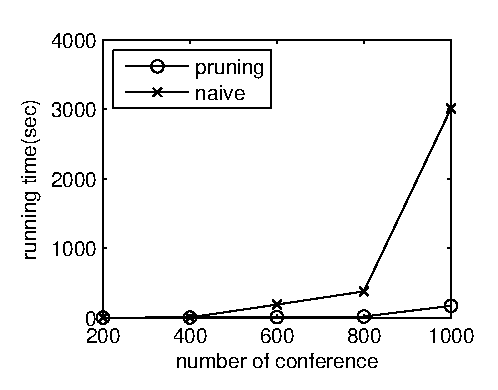
\includegraphics[width=0.7\textwidth]{figs/DBLP}
    \caption{o: Running time with pruning, x: Running time without pruning}
    x-axis: number of labels.
\end{figure}

DBLP Data Set:\\
Graph: 96505 Nodes, 1656732 Edges.\\
    


\section{Experiments of Spatial Skyline Subspace Query}


